\documentclass{article}
\usepackage[utf8]{inputenc}
\usepackage[margin=1in]{geometry}
\usepackage{amsmath, amsfonts, amsthm}
\usepackage{fancyhdr}
\usepackage{multicol}
\usepackage{graphicx}
\usepackage[inline]{enumitem}
\usepackage{wrapfig}
\usepackage[export]{adjustbox}
\graphicspath{ {images/} }
\pagestyle{empty}
\fancyhf{}
\cfoot{\thepage}
\pagenumbering{gobble}

\lhead{MATB42: Assignment \#10}
\rhead{
Poon, Keegan\\
1002423727\\
Apr 3rd 2018}
\newcommand{\norm}[1]{\| #1 \|}
\newcommand{\deriv}[1]{\frac{d}{d #1}}
\newcommand{\parti}[1]{\frac{\partial}{\partial #1}}
\newcommand{\partis}[2]{\frac{\partial #2}{\partial #1}}
\renewcommand{\headrulewidth}{0pt}
\newcommand{\gam}{\boldsymbol{\gamma}}
\newcommand{\divt}{\text{div} \,}
\begin{document}

\thispagestyle{fancy}
\begin{enumerate}
    \item Let $\boldsymbol F$ be a vector field on $\mathbb{R}^3$ given by $\boldsymbol F = (F_1, F_2, F_3)$ where $F_1$, $F_2$, and $F_3$ are $C^1$-functions from $\mathbb{R}^3 \rightarrow \mathbb{R}$
    \begin{enumerate}
        \item Let $\eta$ be the 2-form given by
            \[ \eta = F_3 \, dx \, dy + F_1 \, dy \, dz + F_2 \, dz \, dx \]
            Show that $d\eta = (\divt \boldsymbol F) \, dx \, dy \, dz$
            
            (page 489, \#6)

            \begin{align*} 
                \eta &= F_3 \, dx \, dy 
                + F_1 \, dy \, dz 
                + F_2 \, dz \, dx \\
                d\eta &= d(F_3 \, dx \, dy 
                + F_1 \, dy \, dz 
                + F_2 \, dz \, dx) \\
                &= (dF_3)\, dx \, dy 
                + (dF_1) \, dy \, dz 
                + (dF_2) \, dz \, dx \\
                &= (\parti{x} F_3 \,dx 
                + \parti{y} F_3 \, dy 
                + \parti{z} F_3  \, dz)\, dx \, dy 
                + (dF_1) \, dy \, dz 
                + (dF_2) \, dz \, dx \\
                &= \parti{z} F_3  \, dz \, dx \, dy 
                + (dF_1) \, dy \, dz 
                + (dF_2) \, dz \, dx \\
                &= \parti{z} F_3  \, dx \, dy \, dz 
                + (\parti{x} F_1 \,dx 
                + \parti{y} F_1 \, dy 
                + \parti{z} F_1  \, dz) \, dy \, dz 
                + (dF_2) \, dz \, dx \\
                &= \parti{z} F_3  \, dx \, dy \, dz 
                + \parti{x} F_1 \,dx \, dy \, dz 
                + (dF_2) \, dz \, dx \\
                &= \parti{z} F_3  \, dx \, dy \, dz 
                + \parti{x} F_1 \,dx \, dy \, dz 
                + (\parti{x} F_2 \,dx 
                + \parti{y} F_2 \, dy 
                + \parti{z} F_2  \, dz) \, dz \, dx \\
                &= \parti{z} F_3  \, dx \, dy \, dz 
                + \parti{x} F_1 \,dx \, dy \, dz 
                + \parti{y} F_2 \, dy \, dz \, dx \\
                &= \parti{z} F_3  \, dx \, dy \, dz 
                + \parti{x} F_1 \,dx \, dy \, dz 
                + \parti{y} F_2 \, dx \, dy \, dz \\
                &= \parti{x} F_1 
                + \parti{y} F_2 
                + \parti{z} F_3 \, dx \, dy \, dz 
                = (\divt \boldsymbol F) \, dx \, dy \, dz
            \end{align*} 
        \newpage
        \item Show that $dF_1 \wedge dF_2 \wedge dF_3 
        = (\text{det } D \boldsymbol F ) \, dx \, dy \, dz$
            \[ df = \sum_{i=0}^{n} \partis{x_i}{f} \, dx_i \]
            \begin{align*} 
                dF_1 \wedge dF_2 \wedge dF_3 &= 
                (\partis{x}{F_1} \, dx 
                + \partis{y}{F_1} \, dy 
                + \partis{z}{F_1} \, dz) 
                \wedge (\partis{x}{F_2} \, dx 
                + \partis{y}{F_2} \, dy 
                + \partis{z}{F_2} \, dz) 
                \wedge dF_3 \\
                &= (\partis{x}{F_1} \, dx 
                \wedge (\partis{x}{F_2} \, dx 
                + \partis{y}{F_2} \, dy 
                + \partis{z}{F_2} \, dz) \\
                &\; \; \; \; 
                + \partis{y}{F_1} \, dy 
                \wedge (\partis{x}{F_2} \, dx 
                + \partis{y}{F_2} \, dy 
                + \partis{z}{F_2} \, dz) \\
                &\; \; \; \; 
                + \partis{z}{F_1} \, dz 
                \wedge (\partis{x}{F_2} \, dx 
                + \partis{y}{F_2} \, dy 
                + \partis{z}{F_2} \, dz) ) 
                \wedge dF_3 \\
                &= ((\partis{x}{F_1} \partis{y}{F_2} \, dx \, dy 
                + \partis{x}{F_1} \partis{z}{F_2} \, dx \, dz) \\
                &\; \; \; \; 
                + (\partis{y}{F_1} \partis{x}{F_2} \, dy \, dx 
                + \partis{y}{F_1} \partis{z}{F_2} \, dy \, dz) \\
                &\; \; \; \; 
                + (\partis{z}{F_1} \partis{x}{F_2} \, dz \, dx 
                + \partis{z}{F_1} \partis{y}{F_2} \, dz \, dy))
                \wedge dF_3 \\
                &= ((\partis{x}{F_1} \partis{y}{F_2} 
                - \partis{y}{F_1} \partis{x}{F_2}\, dx \, dy) \\
                &\; \; \; \; 
                + (\partis{y}{F_1} \partis{z}{F_2} 
                - \partis{z}{F_1} \partis{y}{F_2} \, dy \, dz) \\
                &\; \; \; \; 
                + (\partis{z}{F_1} \partis{x}{F_2} 
                - \partis{x}{F_1} \partis{z}{F_2} \, dz \, dx ))
                \wedge (\partis{x}{F_3} \, dx 
                + \partis{y}{F_3} \, dy 
                + \partis{z}{F_3} \, dz) \\
                &= (\partis{z}{F_3} (\partis{x}{F_1} \partis{y}{F_2} 
                - \partis{y}{F_1} \partis{x}{F_2}\, dx \, dy \, dz) \\
                &\; \; \; \; 
                + \partis{x}{F_3} (\partis{y}{F_1} \partis{z}{F_2} 
                - \partis{z}{F_1} \partis{y}{F_2} \, dy \, dz \, dx) \\
                &\; \; \; \; 
                + \partis{y}{F_3} (\partis{z}{F_1} \partis{x}{F_2} 
                - \partis{x}{F_1} \partis{z}{F_2} \, dz \, dx \, dy)) \\
                &=  \partis{x}{F_3} (\partis{y}{F_1} \partis{z}{F_2} 
                - \partis{z}{F_1} \partis{y}{F_2}) \, dx \, dy \, dz \\
                &\; \; \; \; 
                - \partis{y}{F_3} (\partis{x}{F_1} \partis{z}{F_2} 
                - \partis{z}{F_1} \partis{x}{F_2}) \, dx \, dy \, dz \\
                &\; \; \; \; 
                + \partis{z}{F_3} (\partis{x}{F_1} \partis{y}{F_2} 
                - \partis{y}{F_1} \partis{x}{F_2})\, dx \, dy \, dz \\
                &=  \partis{x}{F_3} 
                \begin{vmatrix} \partis{y}{F_1} & \partis{z}{F_1} \\ 
                                \partis{y}{F_2} & \partis{z}{F_2} \end{vmatrix}
                - \partis{y}{F_3} 
                \begin{vmatrix} \partis{x}{F_1} & \partis{z}{F_1} \\ 
                                \partis{x}{F_2} & \partis{z}{F_2} \end{vmatrix}
                + \partis{z}{F_3} 
                \begin{vmatrix} \partis{x}{F_1} & \partis{y}{F_1} \\ 
                                \partis{x}{F_2} & \partis{y}{F_2} \end{vmatrix} 
                                \, dx \, dy \, dz \\
                &=
                \begin{vmatrix}
                    \partis{x}{F_1} & \partis{y}{F_1} & \partis{z}{F_1} \\
                    \partis{x}{F_2} & \partis{y}{F_2} & \partis{z}{F_2} \\
                    \partis{x}{F_3} & \partis{y}{F_3} & \partis{z}{F_3} \\
                \end{vmatrix} \, dx \, dy \, dz
            \end{align*} 
    \end{enumerate}
    \newpage
    \item Let $\omega$ be a $k$-form and let $\eta$ be a $\ell$-form. 
    Find $d(d\omega \wedge \eta - \omega \wedge d\eta)$.
        \begin{align*}
            d(d\omega \wedge \eta - \omega \wedge d\eta) 
            &= d(d\omega \wedge \eta) - d(\omega \wedge d\eta) \\
            &= (d^2 \omega \wedge \eta 
            + (-1)^{k+1} (d \omega \wedge d \eta)) 
            - (d \omega \wedge d \eta + (-1)^k (\omega \wedge d^2 \eta)) \\
            &= (-1)^{k+1} d \omega \wedge d \eta - d \omega \wedge d \eta \\
            &= ((-1)^{k+1} - 1) d \omega \wedge d \eta \\
        \end{align*} 
    \item Determine if $\eta = y \, dx \, dy + xz \, dy \, dz - yz \, dz \, dx$
    is exact. If $\eta$ is exact find a 1-form $\omega$ with $d\omega = \eta$.
    Check if $d\eta = \mathcal{O}$ to see if $\eta$ closed.

    (compare with page 461, \# 22)

    \begin{align*}
        d\eta &= d (y\, dx \, dy + xz \, dy \, dz - yz \, dz \, dx) \\
        &= (dy \, dx \, dy + d(xz)\wedge  dy \, dz - d(yz) \wedge dz \, dx) \\
        &= ((z \, dx + x \, dz)\wedge  dy \, dz 
        - (z\, dy + y \, dz) \wedge dz \, dx) \\
        &= (z \, dx) \wedge dy \, dz - (z\, dy) \wedge dz \, dx \\
        &= z \, dx \, dy \, dz - z \, dx \, dy \, dz = \mathcal{O}\\
    \end{align*}
    Since the polynomials of $x$, $y$ and $z$ defined throughout $\mathbb{R}^3$
    and $\eta$ closed, it is exact. By inspection, 
    \[ \omega = xy \, dy + xyz \, dz \]
    \newpage
    \item
    Evaluate $\displaystyle \iint_S \omega$, where 
    $\omega = z\, dx \, dy + x \, dy \, dz + y \, dz \, dx$ 
    and $S$ is the unit sphere, directly and by the Divergence Theorem.

    (page 489, \#12)

    Directly: 
    
    Parametrize the sphere $S$ as 
    \[ \boldsymbol \Phi (\varphi, \theta) = 
    ( \cos\theta \sin\varphi , \sin\theta \sin\varphi, \cos\varphi)
    \; \text{with }\theta \in [0,2\pi],\, \varphi \in [0,\pi] \]
    \begin{align*}
        \iint_S \omega &= \iint_{\boldsymbol \Phi} z \, dx \, dy 
        + \iint_{\boldsymbol \Phi} x \, dy \, dz 
        + \iint_{\boldsymbol \Phi} y \, dz \, dx \\
        &= \int_0^{2\pi} \int_0^{\pi} 
        \cos \varphi 
        \begin{vmatrix}
        \partis{\varphi}{\cos\theta \sin \varphi} 
        & \partis{\theta}{\cos\theta \sin \varphi} 
        \\ \partis{\varphi}{\sin\theta \sin\varphi} 
        & \partis{\theta}{\sin\theta \sin\varphi} 
        \end{vmatrix} \, d\varphi \, d\theta 
        + \int_0^{2\pi} \int_0^{\pi} \cos\theta \sin\varphi 
        \begin{vmatrix} \partis{\varphi}{\sin\theta \sin\varphi} 
        & \partis{\theta}{\sin\theta \sin\varphi} 
        \\ \partis{\varphi}{\cos \varphi} 
        & \partis{\theta}{\cos \varphi} 
        \end{vmatrix}\, d\varphi \, d\theta \\
        & \; \; \; \; 
        + \int_0^{2\pi} \int_0^{\pi} \sin\theta \sin\varphi 
        \begin{vmatrix} \partis{\varphi}{\cos \varphi} 
        & \partis{\theta}{\cos \varphi} 
        \\ \partis{\varphi}{\cos\theta \sin\varphi} 
        & \partis{\theta}{\cos\theta \sin\varphi}
        \end{vmatrix}\, d\varphi \, d\theta \\
        &= \int_0^{2\pi} \int_0^{\pi} \cos \varphi 
        \begin{vmatrix}\cos \theta \cos \varphi 
        & - \sin \theta \sin \varphi  
        \\ \sin \theta \cos \varphi 
        & \cos \theta \sin \varphi 
        \end{vmatrix} \, d\varphi \, d\theta 
        + \int_0^{2\pi} \int_0^{\pi} \cos\theta \sin\varphi 
        \begin{vmatrix} \sin \theta \cos \varphi 
        & \cos \theta \sin \varphi \\ -\sin \varphi 
        & 0 \end{vmatrix}\, d\varphi \, d\theta \\
        & \; \; \; \; 
        + \int_0^{2\pi} \int_0^{\pi} \sin\theta \sin\varphi 
        \begin{vmatrix} -\sin \varphi 
        & 0 \\ \cos \theta \cos \varphi 
        & - \sin \theta \sin \varphi \end{vmatrix}\, d\varphi \, d\theta \\
        &= \int_0^{2\pi} \int_0^{\pi} 
        \sin \varphi \cos^2 \varphi \, d\varphi \, d\theta 
        + \int_0^{2\pi} \int_0^{\pi} \cos^2\theta \sin^3\varphi 
        + \sin^2\theta \sin^3\varphi \, d\varphi \, d\theta \\
        &= \int_0^{2\pi} \int_0^{\pi} \sin \varphi (\cos^2 \varphi 
        + \sin^2 \varphi) \, d\varphi \, d\theta  \\
        &= \int_0^{2\pi} \int_0^{\pi} \sin \varphi  \, d\varphi \, d\theta  \\
        &= 2\pi \bigg[ -\cos \varphi\bigg]_0^{\pi} = 2\pi \\
    \end{align*}
    Divergence Theorem:
    \[ d\omega = dz \, dy \, dx 
    + dx \, dy \, dz + dy dz dx = 3 \, dx \, dy \, dz \]
    \begin{align*}
        \iint_S \omega &= \iiint_R d \omega \\
        &= 3 \int_0^{2\pi} \int_0^{\pi} \int_0^1 
        \rho^2 \sin(\varphi) \, d\rho \, d\varphi \, d\theta \\
        &= \int_0^{2\pi} \int_0^{\pi} \sin(\varphi) \, d\varphi \, d\theta \\
        &= 2\pi \bigg[ -\cos \varphi\bigg]_0^{\pi} = 2\pi \\
    \end{align*}

    \newpage
    \item Compute $\displaystyle \int_S \omega$ and use symbolic algebra 
    software to sketch $S$ in each of the following.
    \begin{enumerate}
        \item $\omega = xz \, dx \, dy + x^2 \, dy \, dz + dy \, dz \, dx$
  
        S is the upper hemisphere $x^2 + y^2 + z^2 = 4$, $z \geq 0$ with 
        $\boldsymbol n$ pointing upward.
        
        Close it with the disk of radius 2 on the $xy$-plane to apply divergence 
        theorem
        \[ \boldsymbol \Phi(\theta, r) = 
        (r \cos \theta, r \sin \theta, 0),\; 
        r \in [0,2],\, \theta \in [0, 2\pi] \]
        \begin{align*}
            dx\, dy &= 
            \begin{vmatrix} -r\sin \theta & \cos \theta \\ 
                             r \cos \theta &  \sin \theta 
            \end{vmatrix} = -2r \\
            &\text{ Which is negative, 
            so correct orientation for normal pointing down.} \\
            dy\, dz &= 0 \text{ Since $z$ is 0} \\
            dz\, dx &= 0 \\
            \overset{\text{Div Thm}}{\implies} \iint_S \omega &= 
            \iiint_R d\omega - \iint_{\boldsymbol \Phi} \omega \\
            &\text{But } z = 0 \implies xz \, dx \, dy = 0 
            \implies \iint_{\boldsymbol \Phi} \omega = 0 \\
            d\omega &= x \, dx \, dy \, dz + 2x \, dx \, dy \, dz 
            = 3x \, dx \, dy \, dz \\
            \iiint_R d\omega &= \int_0^{2} \int_0^{2\pi} \int_0^{\frac{\pi}{2}}
            3(\rho \sin \varphi \cos \theta) \rho^2 \sin \varphi 
            \, d\varphi \, d\theta \, d\rho \\
            &= 0 \text{ Since integrating cos over full period} \\
            \implies \int_S \omega = 0
        \end{align*}

        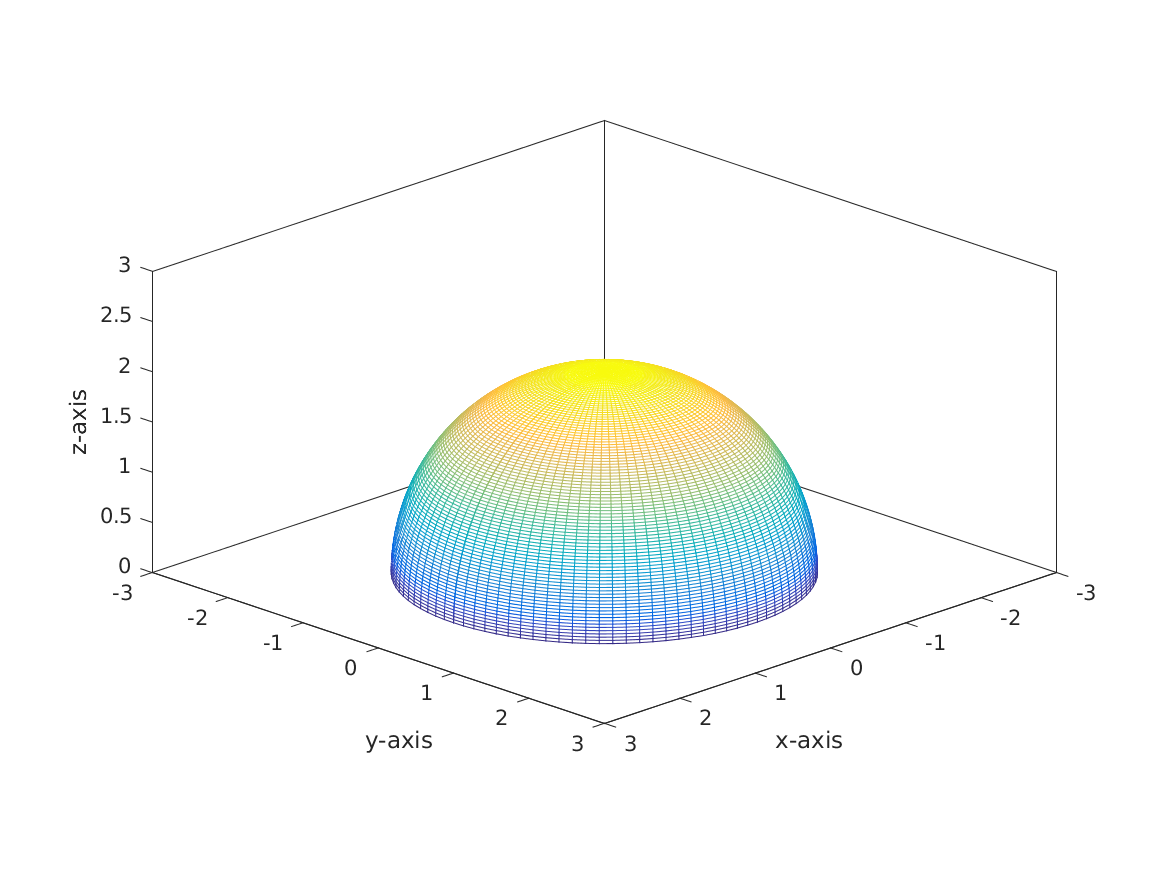
\includegraphics[width=0.75\textwidth,center]{b42-a10-5a}

        \newpage
        \item $\omega = z \, dx \, dy + x \, dy \, dz + y \, dz \, dx$

        $S$ is the part of the plane $x+y+z = 1$ which lies in the first 
        octant oriented by the unit normal which points upward.

        Use the natural parametrization for $S$:
        \[ \boldsymbol \Phi (x, y) = (x, y, 1 - x - y),\; 
        x \in [0,1],\, y \in [0, 1-x] \]
        \begin{align*}
            dx\, dy &= \begin{vmatrix} 1 & 0 \\ 0 & 1 \end{vmatrix} > 0 
            \, \forall x,y \implies \text{ Correct orientation} \\
            \int_S \omega &= 
            \int_0^1 \int_0^{1-x} (1 - x - y) 
            + x\begin{vmatrix} 0 & 1 \\ -1 & -1 \end{vmatrix}  
            + y\begin{vmatrix} -1 & -1 \\ 1 & 0 \end{vmatrix} \, dy \,dx \\
            &= \int_0^1 \int_0^{1-x} 1 \, dy \,dx = \int_0^1 1 - x \,dx \\
            &= 1 - \frac{1}{2} = \frac{1}{2} 
        \end{align*}

        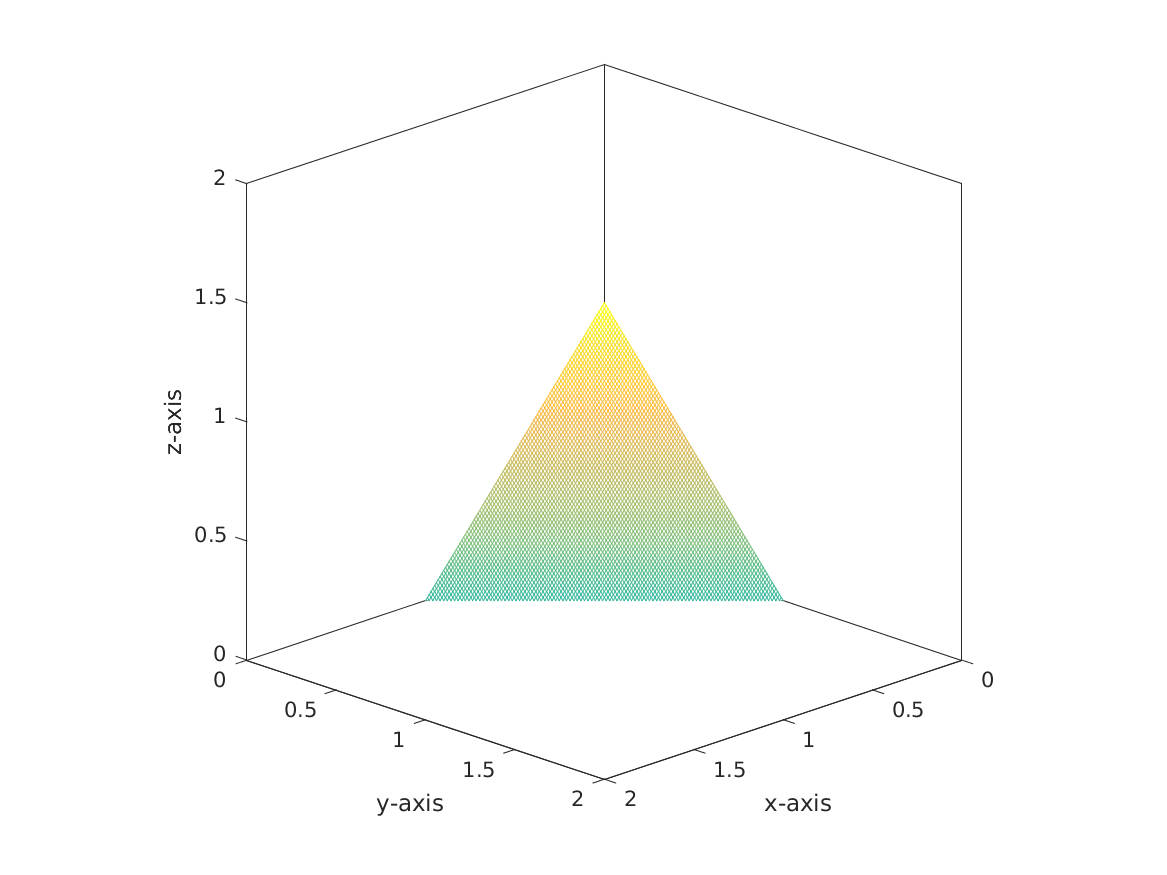
\includegraphics[width=0.75\textwidth,center]{b42-a10-5b}

        \newpage
        \item $\omega  = xz \, dx \, dy + y \, dx \, dz + z^2 \, dy \, dz$
        
        $S$ is the part of the cone $z = \sqrt{x^2 + y^2}$ between $z=1$ 
        and $z=3$,  oriented by the unit normal with negative $z$-component.
        \[ \boldsymbol \Phi (\theta, r) = 
        (r\cos \theta, r\sin \theta, r) 
        ,\; r \in [1,3] ,\, \theta \in [0,2\pi] \]
        \begin{align*}
            dx\, dy &= 
            \begin{vmatrix} -r\sin \theta & \cos \theta 
            \\ r\cos \theta & \sin \theta \end{vmatrix} = -r < 0 
            \text{ for } r > 1 \\
            dy\, dz &= 
            \begin{vmatrix}  r\cos \theta & \sin \theta \\ 0 & 1\end{vmatrix} 
            = r \cos \theta\\
            dz\, dx &= 
            \begin{vmatrix}  0 & 1 \\ -r\sin \theta & \cos \theta \end{vmatrix}
            = r \sin \theta\\
            \implies \omega &= 
            (r \cos \theta)(r)(-r) - (r \sin \theta)(r \sin \theta) 
            + (r)^2(r \cos \theta) \\
            &= -r^2 \sin^2 \theta = 
            -r^2\bigg( \frac{1}{2} - \frac{\cos(2\theta)}{2} \bigg) \\
            \implies \int_S \omega &= \int_1^3 \int_0^{2\pi} 
            -r^2\bigg( \frac{1}{2} - \frac{\cos(2\theta)}{2} \bigg) 
            \, d\theta \, dr \\
            &= \int_1^3 -r^2\pi \, dr = -\pi \bigg[ \frac{r^3}{3} \bigg]_1^3 
            = -\frac{26\pi}{3}\\
        \end{align*}

        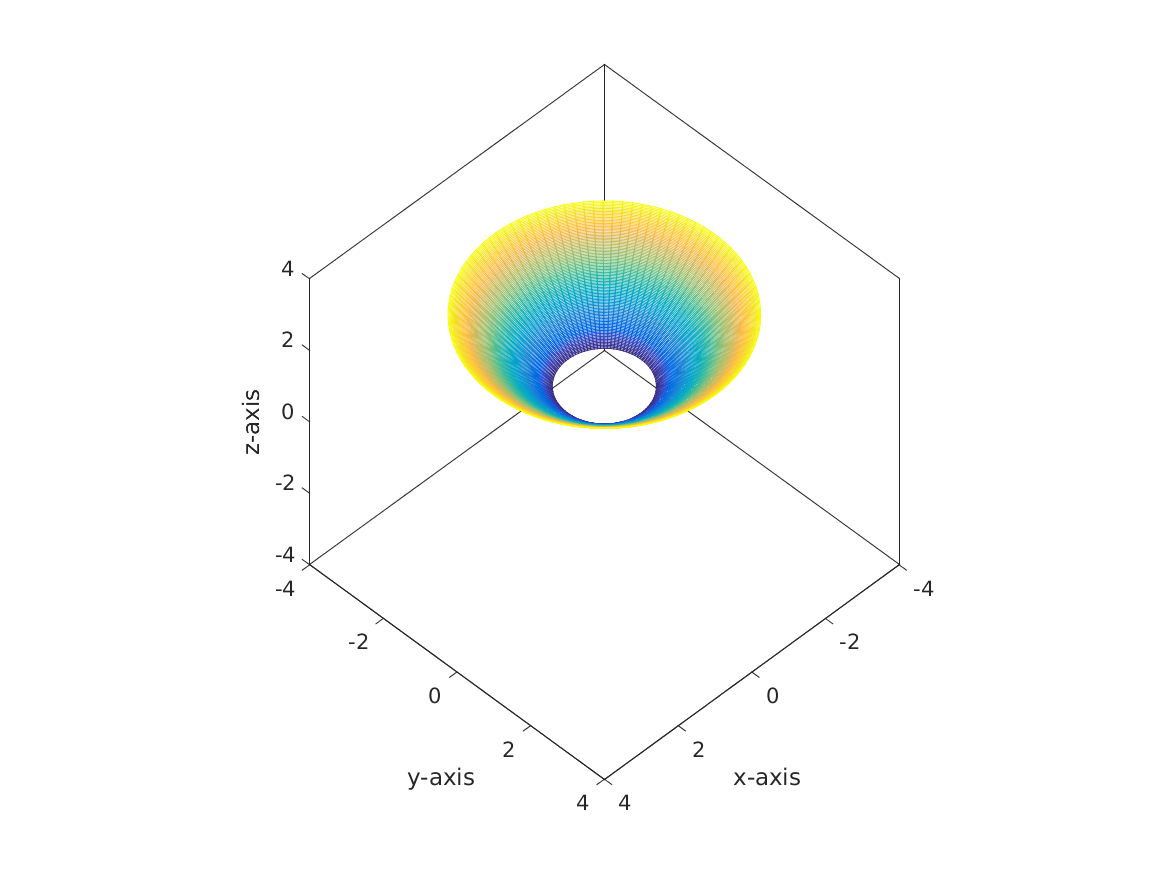
\includegraphics[width=0.75\textwidth,center]{b42-a10-5c}

        \newpage
        \item $\omega = z \, dx \, dy + y \, dy \, dz$
        
        $S$ is the oriented surface given by the parametrization

        $\Phi (u,v) = (u+v, uv^2, u^2 + v^2),\, 0 \leq u \leq 1,\, 0\leq v \leq 1$.

            \[dx \, dy 
            = \begin{vmatrix} 1 & 1 \\ v^2 & 2uv \end{vmatrix} 
            = 2uv - v^2 ,\; \; dy \, dz 
            = \begin{vmatrix} v^2 & 2uv \\ 2u & 2v \end{vmatrix} 
            = 2v^3 - 4 u^2v \]
        \begin{align*}
            \iint_S \omega &= \int_0^1 \int_0^1 (u^2 + v^2)(2uv - v^2) 
            + (uv^2)(2v^3 - 4u^2v) \, du \, dv \\
            &= \int_0^1 \int_0^1 (2u^3v - u^2v^2) + (2uv^3 - v^4) 
            + (2uv^5 - 4u^3v^3) \, du \, dv \\
            &= \int_0^1 \frac{v}{2} - \frac{v^2}{3} + v^3 - v^4 
            + v^5 - v^3 \, du \, dv \\
            &= \int_0^1 \frac{v}{2} - \frac{v^2}{3} - v^4 + v^5 \, du \, dv \\
            &= \frac{1}{4} - \frac{1}{9} - \frac{1}{5} + \frac{1}{6}  
            = \frac{19}{180} \\
        \end{align*}

        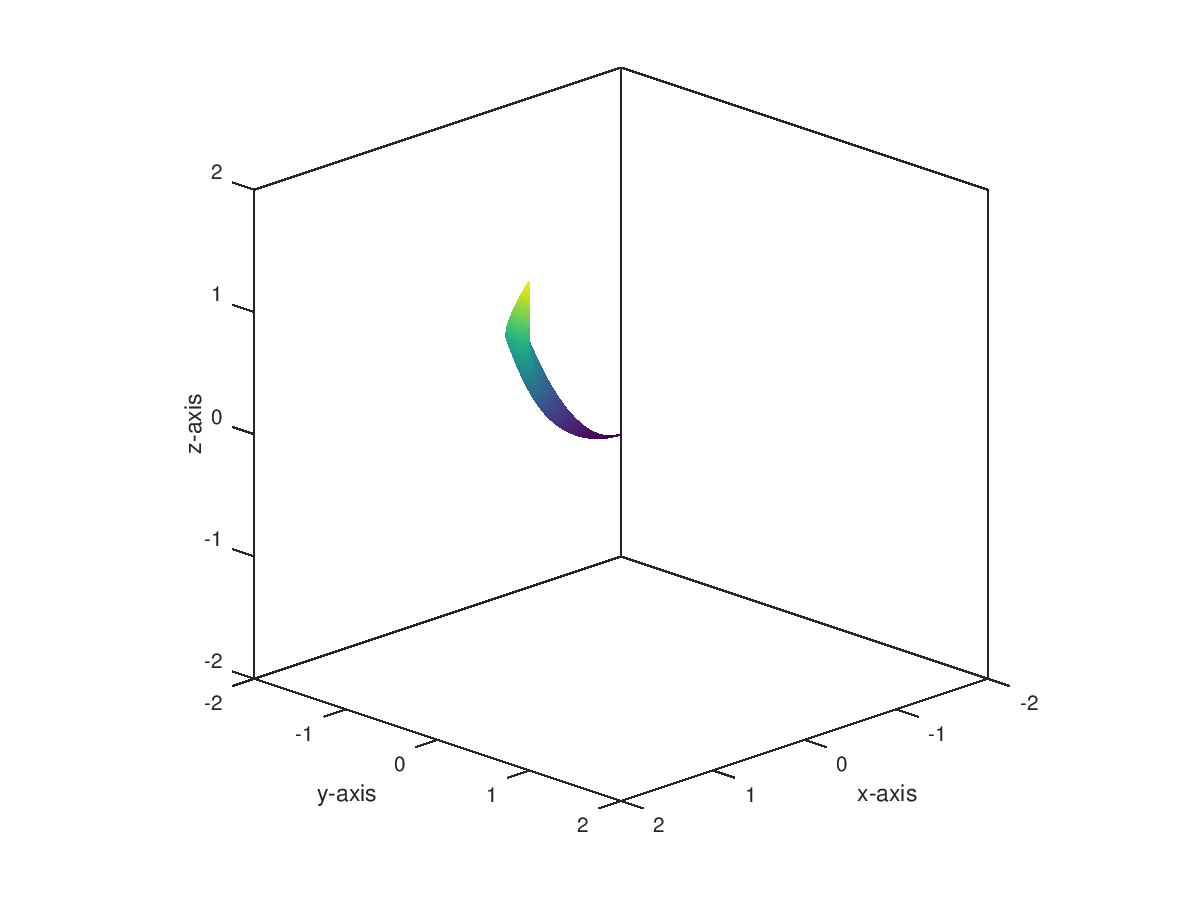
\includegraphics[width=0.75\textwidth,center]{b42-a10-5d}
    \end{enumerate}

    \newpage
    \item Verify Stokes' theorem by direct calculation of both sides when 
    the surface $S$ is the piece of the paraboloid $z= x^2 + y^2 - 4$ with 
    $z \leq 0$, oriented by the downward pointing unit normal, and $\omega 
    = (2y-z)\, dx + (x + y^2 - z)\, dy + (4y-3x)\, dz$.

    As part of your solution, provide a sketch showing the appropriate 
    orientations. (For this question you may draw the sketch by hand 
    or use symbolic algebra software.)

        Stokess' Theorem states that:
        \[ \int_{\partial_S} \omega = \int_S d\omega \]

        Calculation of $\displaystyle \int_{\partial_S} \omega $

        The boundary curve of the plane is the circle at $z = 0$ with radius 
        $2$. Since the normal vector is downward pointing, the curve is 
        parametrized clockwise. So parametrize the curve as 
        $\boldsymbol \gamma(\theta) = (-2\cos \theta, 2\sin \theta, 0)$
        \begin{align*}
            &\int_0^{2\pi} (2(2\sin\theta) - 0)(2\sin \theta) 
            + ((-2\cos \theta) 
            + (2\sin \theta)^2 - 0)(2\cos \theta) \, d\theta \\
            &= \int_0^{2\pi} 8 \sin ^2 \theta - 4 \cos ^2 \theta 
            + 8 \sin^2 \theta \cos \theta \, d \theta \\
            &= \int_0^{2\pi} 4(1 - \cos(2\theta)) - 2 (1 + \cos(2\theta)) 
            + 8 \sin^2 \theta \cos \theta \, d \theta \\
            &= \int_0^{2\pi} 2 + 8 \sin^2 \theta \cos \theta \, d \theta \\
            &= 4\pi + \bigg[\frac{8\sin^3\theta}{3}\bigg]_0^{2\pi} = 4\pi
        \end{align*}

        Calculation of $\displaystyle \int_{S} d\omega$
        
        (Using the parametrization 
        $\boldsymbol \Phi (\theta,r) 
        = (r\cos \theta, r\sin \theta, r^2 - 4),\; 
        r \in [0, 2],\, \theta \in [0, 2\pi])$
        \[ dx\, dy = 
        \begin{vmatrix} -r\sin\theta & \cos \theta \\
                         r \cos \theta & \sin \theta 
        \end{vmatrix} = -r\]
        So the orientation is in the correct direction.
        \begin{align*}
            d\omega &= d(2y-z)\, dx + d(x+y^2-z)\, dy + d(4y -3x)\, dz \\
            &= (2\, dy - \,dz) \wedge dx 
            + (dx - dz) \wedge dy 
            + (4 \, dy -  3\, dx) \wedge dz \\
            &= -2\, dx\, dy - \,dz \, dx + dx \, dy + dy \, dz 
            + 4 \, dy \, dz +  3\, dz \, dx \\
            &= -\, dx\, dy + 5 \, dy \, dz +  2\, dz \, dx \\
            \implies \int_S d\omega &= \int_0^{2\pi} \int_0^2 
            - \begin{vmatrix} -r \sin\theta & \cos \theta \\ 
                               r \cos \theta & \sin \theta \end{vmatrix}
            + 5 \begin{vmatrix} r\cos \theta & \sin \theta \\ 
                                0 & 2r \end{vmatrix}
            + 2 \begin{vmatrix} 0 & 2r \\ 
                               -r\sin\theta & \cos \theta \end{vmatrix} 
            \, dr \, d\theta \\
            &= \int_0^{2\pi} \int_0^2 r + 5 (2r^2\cos \theta) 
            + 2(2r^2 \sin \theta) \, dr \, d\theta\\
            &= 2\pi \int_0^2 r \, dr = 4\pi \\
        \end{align*} 

    \newpage
    \item Let $\omega = yz\, dx - xz \, dy + xy \, dz$ and 
    let $\boldsymbol \gamma(t) = (2\cos t, 2\sin t, 4),\, 0 \leq t \leq 2\pi$.

        \begin{align*}
            d\omega &= d(yz) \wedge dx - d(xy) \wedge dy + d(xy) \wedge dz \\
            &= (z \,dy + y\, dz)\wedge dx - (z \, dx + x \, dz) \wedge dy + 
            (y \, dx + x \, dy) \wedge dz \\
            &= z \,dy \, dx + y\, dz \, dx - z \, dx \, dy - x \, dz \, dy + 
            y \, dx \, dz + x \, dy \, dz \\
            &= -2z \,dx \, dy  + 2x \, dy \, dz \\
        \end{align*} 
    \begin{enumerate}
        \item Let $S$ be the piece of the surface $z = x^2 + y^2$ with 
            $z \leq 4$. Use Stokes' theorem to give an integral over $S$ 
            which is equivalent to $\displaystyle \int_{\boldsymbol \gamma} 
            \omega$. Verify by directly computing both integrals.

            Note that the boundary of $S$ at $z = 4$ is $\boldsymbol \gamma$.
            This means that, if the orientation is compatible, Stokes' theorem 
            will apply. Since the orientation of the curve is counter 
            clockwise, the normal vector should be pointing up for the surface.
            
            To parametrize $S$, use a similar parametrization to the one in 
            question 6.
            \[ \boldsymbol \Phi (r, \theta)
            = (r\cos \theta, r\sin \theta, r^2),\;
            r \in [0,2] ,\, \theta \in [0,2\pi] \]
            The normal vector is also oriented correctly.
            \[ dx\, dy = \begin{vmatrix} \cos \theta & -r\sin \theta \\ 
            \sin \theta & r \cos \theta \end{vmatrix} = r \geq 0 \] 
            \[ \overset{\text{Stokes' Thm}}{\implies} 
            \int_{\partial S = \boldsymbol \gamma} \omega = \int_S d \omega \]
            \begin{align*}
                \int_{\boldsymbol \gamma} \omega &= \int_0^{2\pi} 
                (2\sin t)(4)(-2\sin t) - (2\cos t)4(2\cos t) \, dt \\
                &= \int_0^{2\pi}  -16(\sin ^2 t + \cos ^2 t) \, dt \\
                &= \int_0^{2\pi} -16 \, dt  = -32 \pi\\
                \int_S d \omega &= \int_0^2 \int_0^{2\pi} -2(r^2)(r) 
                + 2(r \cos \theta)
                \begin{vmatrix} \sin \theta & r \cos \theta \\
                                  2r & 0
                \end{vmatrix} \, d\theta \, dr \\
                \int_S d \omega &= \int_0^2 \int_0^{2\pi} -2(r^2)(r) 
                - 4(r^3 \cos \theta) \, d\theta \, dr \\
                \int_S d \omega &= \int_0^2 \int_0^{2\pi} -2(r^2)(r) 
                - 2(r^3(1 + \cos (2 \theta) )\, d\theta \, dr \\
                &= \int_0^2 -4 \pi r^3 \, d\theta \, dr \\
                &= -(2^2) \pi \bigg[ \frac{r^4}{2^2} \bigg]_0^2 = -32 \pi \\
            \end{align*} 

        \item Let $S'$ be the part of the plane $z=4$ with $x^2 + y^2 \leq 4$.
        Use Stokes' theorem to give an integral over $S'$ which is equivalent 
        to $\displaystyle \int_{\gamma} \omega$. Verify by direct computation.
        
            Note that the disk $S'$ can be parametrized as $\boldsymbol \Phi
            (r, \theta) = (r \cos \theta, r \sin \theta, 4),\; r \in [0,2],\,
            \theta \in [0,2\pi]$ as we have that
            \[ dx\, dy = \begin{vmatrix} \cos \theta & -r\sin \theta \\ 
            \sin \theta & r \cos \theta \end{vmatrix} = r \geq 0 \] 
            Also, the same conditions hold for the normal vector as the curve
            at the boundary has not changed. ($S'$ also intersects with the 
            $z=4$ plane at the radius 2 disk.

            \begin{align*}
                \int_{\boldsymbol \gamma} \omega &= \int_0^{2\pi} 
                (2\sin t)(4)(-2\sin t) - (2\cos t)4(2\cos t) \, dt \\
                &= \int_0^{2\pi}  -16(\sin ^2 t + \cos ^2 t) \, dt \\
                &= \int_0^{2\pi} -16 \, dt  = -32 \pi\\
                \int_{S'} d \omega &= \int_0^2 \int_0^{2\pi} -2(4)(r) + 0 \,
                d\theta \, dr \\
                &= \int_0^2 -16 \pi r \, d\theta \, dr \\
                &= -16 \pi \bigg[ \frac{r^2}{2} \bigg]_0^2 = -32 \pi \\
            \end{align*} 

        \item Can you give another explanation as to why the integrals you 
        get over $S$ and $S'$ should have the same value?

    \end{enumerate}
    
    \newpage
    \item Let $\boldsymbol F (x,y,z) = (e^{z^2}, 4z-y, 8x \sin y)$. 
    Find $\displaystyle \int_S (\nabla \times \boldsymbol F)\cdot d\boldsymbol 
    S$ where $S$ is the unit sphere oriented with the outward normal.

    \newpage
    \item 
    \begin{enumerate}
        \item Marsden \& Tromba, page 451, \# 13.

            Let $S$ be the capped cylindrical surface shown in Figure 1. 
            $S$ is the union of two surfaces, $S_1$ and $S_2$, where $S_1$ 
            is the set of $(x,y,z)$ with $x^2 + y^2 = 1$, $0 \leq z \leq 1$, 
            and $S_2$ is the set of $(x,y,z)$ with $x^2 + y^2 + (z-1)^2 = 1$,
            $z \geq 1$. Set $\boldsymbol F (x,y,z) = (zx + z^2y + x) 
            \boldsymbol i + (z^3yx + y)\boldsymbol j + z^4x^2\boldsymbol k$.
            Compute $\displaystyle \iint_S (\nabla \times \boldsymbol F) \cdot
            d \boldsymbol S$. (\textsc{Hint}: Stokes' theorem holds for this
            surface.)


        \item Marsden \& Tromba, page 451, \# 15.

            Evaluate the integral $\displaystyle \iint_S (\nabla \times 
            \boldsymbol F) \cdot d \boldsymbol S$, where $S$ is the portion
            of the surface of a sphere defined by $x^2 + y^2 + z^2 = 1$ and
            $x + y + z = \geq 1$, and where $\boldsymbol F = \boldsymbol r
            \times ( \boldsymbol i + \boldsymbol j + \boldsymbol k),\, 
            \boldsymbol r = x \boldsymbol i + y \boldsymbol j + z \boldsymbol
            k.$
        \item Use symbolic algebra software to sketch the surfaces in parts (a) and (b).
    \end{enumerate}
    
    \newpage
    \item 
    \begin{enumerate}
        \item Let $\boldsymbol F$ and $\boldsymbol G$ be vector fields on 
        $\mathbb{R}^3$ and let $f : \mathbb{R}^3 \rightarrow \mathbb{R}$.
        Verify the following identities.
        \begin{enumerate}[label=(\roman*)]
            \item $\divt (\boldsymbol F \times \boldsymbol G) 
            = \boldsymbol G \cdot \text{curl} \, \boldsymbol F 
            - \boldsymbol F \cdot \text{curl} \, \boldsymbol G.$
            \item curl$(f \boldsymbol F) 
            = f \text{curl} \boldsymbol F 
            + (\text{grad}\, f) \times \boldsymbol F$.
        \end{enumerate}
        \item Let $R$ be a closed region in $\mathbb{R}^3$ with boundary 
        $\partial R$. Prove the identity
        \[\int_{\partial R} ( \boldsymbol F \times \text{curl} \boldsymbol G) 
        \cdot \, d \boldsymbol S = 
        \int_R(\text{curl} \boldsymbol F ) 
        \cdot (\text{curl} \boldsymbol G) \, dV 
        - \int_R \boldsymbol F 
        \cdot \text{curl}(\text{curl} \boldsymbol G ) \, dV\]
        (page 490, \#2)
    \end{enumerate}
\end{enumerate}
\end{document}
